\chapter{Demos clásicas}

\section{Fuego}

\subsection{Investigación inicial}

Una demo que simule un efecto de fuego se podría considerar algo así como el "hola mundo" de la demoscene. Es un ejercicio sencillo con un resultado final bastante espectacular.\\

Tras una búsqueda de información inicial, pude encontrar también dos sitios diferentes en los que se explicaba cómo crear un efecto de fuego.\\ 

En el canal de YouTube de Creature Mann\footnote{\url{https://www.youtube.com/user/kjlg74/featured}} se explica la base teórica para crear un efecto de fuego sencillo\footnote{\url{https://www.youtube.com/watch?v=_SzpMBOp1mE}}. A este vídeo le siguen un par de vídeos de este mismo creador\footnote{\url{https://www.youtube.com/watch?v=iezD8B1ym3w}}\footnote{\url{https://www.youtube.com/watch?v=206TEPBOnLc}} en los que itera sobre el efecto anteriormente creado, añadiendo complejidad (como la posibilidad de controlar la dirección del fuego o trazar un camino que se prende fuego). Por desgracia, los enlaces provistos al código que estos vídeos muestran están caídos, por lo que el código no es accesible. No obstante, la parte argumentablemente más importante, la explicación teórica del efecto, se hace en el primer vídeo.\\

Otra página que ofrece una descripción muy buena del efecto es Lode's Computer Graphics Tutorial\footnote{\url{https://lodev.org/cgtutor/fire.html}}. Esta página sí que aporta código, aunque decidí ignorar la implementación (para evitar que condicionara mi propio desarrollo) y centrarme únicamente en la explicación teórica que se ofrecía, muy similar a la del vídeo anterior aunque más técnica.\\

\subsection{Planteamiento formal}

El fuego es un efecto muy sencillo tanto a nivel teórico como de implementación. Consiste en la convolución de una matriz como la de la figura [\ref{fig:firematrix}] a lo largo de una matriz que tan sólo contiene valores en su fila inferior. Al aplicar esta operación de abajo a arriba, se obtiene un conjunto de valores [\ref{fig:fire_whitegrid}] que al ser asociados a un set concreto de colores [\ref{fig:fire_colouredgrid}], dan una sensación similar al fuego.\\

\begin{figure}
	\begin{equation}
		\begin{bmatrix}
			0 & 0 & 0 \\
			0 & 0 & 0 \\
			\frac{1}{3} & \frac{1}{3} & \frac{1}{3}
		\end{bmatrix}
	\end{equation}
	\caption{Matriz de convolución para generar efecto de fuego}
	\label{fig:firematrix}
\end{figure}

Otra forma de entender esta operación es la siguiente: el valor de cada píxel se deduce de la media del valor de los tres píxeles adyacentes por debajo de él. Para que este efecto se produzca de forma efectiva, la fila inferior de píxeles se suele rellenar con valores aleatorios. De esta forma, la tendencia natural de este modelo es la de disiparse.\\

El único caso en el que no se produciría disipación sería en el que todos los valores de la fila inferior se inicializaran al máximo (en cuyo caso todos los píxeles acabarían con el mismo valor). Para cualquier otra situación, se produce una atenuación progresiva de los valores. 

\begin{figure}[h]
	\centering
	\begin{subfigure}[b]{0.45\textwidth}
		\centering
		\includegraphics[width=5.09cm]{archivos/fire_whitegrid}
		\caption{Valores resultantes tras convolucionar iterativamente la matriz [\ref{fig:firematrix}] por una matriz de ceros, con valores solo en la fila inferior}
		\label{fig:fire_whitegrid}
	\end{subfigure}
	\begin{subfigure}[b]{0.45\textwidth}
		\centering
		\includegraphics[width=6cm]{archivos/fire_colouredgrid}
		\caption{Efecto resultante de asociar determinados rangos de valores a un set de colores preestablecido}
		\label{fig:fire_colouredgrid}
	\end{subfigure}
\end{figure}

Dado el comportamiento descrito, será necesario realizar los siguientes pasos:
\begin{itemize}
	\item Implementar una forma de realizar degradados (o mapas de color)
	\item Reservar e inicializar una matriz a cero, con valores aleatorios en su fila inferior
	\item Implementar el comportamiento de convolución de la matriz [\ref{fig:firematrix}]
\end{itemize}

\subsection{Implementación}

Para poder crear degradados, se crea la función \emph{GenerateGradient} que dado un conjunto de \emph{ColourStamp} y un tamaño, interpola los valores de colores pasados para generar un degradado continuo en \emph{colourMap}.\\

\begin{lstlisting}[style=C-color, caption={Método para crear gradientes de color},label=cod:generateGradient]
static void GenerateGradient(std::vector<ColourStamp> colours, Pixel* colourMap, int colourMapSize);
\end{lstlisting}

\emph{ColourStamp} (marca de color) es una estructura formada por dos variables: un color y un número decimal (que puede oscilar entre 0 y 1). Este número señala la posición de este color en el gradiente o mapa de color, siendo 0 el inicio y 1 el final. 

\begin{figure}[h]
	\centering
	\includegraphics[width=12cm]{archivos/colourGradient}
	\caption{Degradado en 32 celdas dadas 5 marcas de color}
	\label{fig:colourGradient}
\end{figure}

De este modo, si llamamos a la función \emph{GenerateGradient} con los valores para las marcas de color representados en la figura [\ref{fig:colourGradient}] y pasamos un \emph{array} con capacidad para 32 valores, este método producirá un set de colores similar al ilustrado. Esto se hace mediante una interpolación lineal entre los valores que se pasan, creando un degradado de forma progresiva.\\

Una vez tenemos implementado este método, ya podemos crear un degradado de colores de forma sencilla y cómoda, automatizando el proceso de crear un mapa de color para el fuego.\\

Para nuestra implementación, en lugar de asignar a un rango de valores un color específico, asignaremos un color por valor entero. Esto permitirá un resultado más realista, al disponer de una mayor cantidad de colores. Cada celda de nuestra matriz de valores estará formada por un byte. Esto implica que cada celda podrá tener 256 valores distintos, y que por tanto necesitaremos generar un degradado que nos devuelva 256 colores.\\

Creamos un mapa de valores de un byte de tamaño, lo inicializamos a 0 e inicializamos aleatoriamente algunas de las celdas de la fila inferior a su valor máximo (255).\\

\begin{lstlisting}[style=C-color, caption={Creación e incialización del mapa de valores},label=cod:screenMapping,escapechar=|]
screenMapping = new unsigned char[width * height];

for (int i = width * (height - 1), n = width * height; i < n; i++)
{
    if (Fast::Rand() % 10 == 0)|\label{line:fastRand}|
    {
        screenMapping[i] = 255;
    }
}
\end{lstlisting}

Como podemos ver en la línea [\ref{line:fastRand}], hacemos uso de una función propia para la generación de números aleatorios. Esta función está basada en el algoritmo \emph{Xorshift}\footnote{\url{https://en.wikipedia.org/wiki/Xorshift}} de George Marsaglia. La apromaximación usada está basada en una respuesta de \emph{StackOverflow}\footnote{\url{https://stackoverflow.com/questions/1640258/need-a-fast-random-generator-for-c}}.\\

La decisión de usar nuestro propio generador de números aleatorios se debe a que el usualmente provisto por la STL \footnote{\url{https://en.wikipedia.org/wiki/Standard_Template_Library}} es innecesariamente lento y complejo para nuestras necesidades. Para nuestro caso, no necesitamos un algoritmo que pase todos los tests de aleatoriedad\footnote{\url{https://es.wikipedia.org/wiki/Pruebas_de_aleatoriedad}}, con tal de que sea suficientemente "aleatorio al ojo" y sea rápido, nos basta.\\

Una vez hecho esto, tan sólo queda implementar el algoritmo principal, que cree el efecto de fuego sobre el mapa de valores previamente creado, de acorde a la operación descrita en la figura [\ref{fig:firematrix}] y asocie dichos valores con un color generado por la función \emph{GenerateGradient} [\ref{cod:generateGradient}].\\

\begin{lstlisting}[style=C-color, caption={Algoritmo básico de efecto de fuego},label=cod:simpleFire,escapechar=|]
for (int i = width * (height - 1); i >= 0; i--)
{
    int lowerCell = width + i;|\label{line:simpleFire1}|
    int newCellValue = screenMapping[i] = (screenMapping[lowerCell + 1] + screenMapping[lowerCell] + screenMapping[lowerCell - 1]) / 3.0;|\label{line:simpleFire2}|
    pixels[i] = colourMap[newCellValue];|\label{line:simpleFire3}|
}
\end{lstlisting}

En el código [\ref{cod:simpleFire}] podemos  ver el algoritmo de generación de fuego en su forma más simple. Recorremos la pantalla de abajo a arriba y operamos por cada píxel. En la línea [\ref{line:simpleFire1}] obtenemos, para una posición dada en el mapa de valores, la posición del valor inmediatamente por debajo del mismo. Una vez obtenida esta posición, operamos haciendo la media usando su valor y los adyacentes. Guardamos el resultado como nuevo valor y usamos a la vez este nuevo valor para asociar un nuevo color al píxel en pantalla (línea [\ref{line:simpleFire3}]). Los valores más altos (255) representan tonos blancos y/o amarillentos, mientras que los valores intermedios representarán valores rojizos y los valores más bajos tendrán asociados colores más oscuros.\\

El resultado de aplicar este algoritmo resulta en una imagen estática y de aspecto poco realista [\ref{fig:fire_simple}], pero que ya se empieza a parecer al efecto que buscamos.\\

\begin{figure}[h]
	\centering
	\includegraphics[width=8cm]{archivos/fire_simple}
	\caption{Fuego estático, usando el algoritmo en [\ref{cod:simpleFire}]}
	\label{fig:fire_simple}
\end{figure}

\subsection{Refinamiento}

Una vez tenemos el efecto de fuego a nivel básico, es el momento de iterar sobre la idea y ver cómo mejorarla. A continuación se listan y explican las medidas tomadas, mostradas en el orden en que se aplicaron:

\begin{itemize}
	\item \textbf{Hacer fuego dinámico}: una vez obtenido un fuego estático, era el momento de darle movimiento, y que tuviera un efecto realista. Inicialmente probé con una técnica que se sugería en algunos de los tutoriales que había seguido: en lugar de dibujar el fuego de abajo a arriba, dibujarlo de arriba a abajo y aleatorizar la base, de forma que las variaciones en el fuego derivaran a partir de las variaciones en la base.
	
	El resultado no me dejó convencido. Cuando uno observa un fuego o una llama, la parte más cambiante del fuego no es la base, la base es siempre estable y es la parte superior la que más titila / oscila. Por tanto no tenía para mí sentido generar dinamismo aleatorizando la base.
	
	Una llama se caracteriza a menudo por tener una intensidad variante, y fue esto lo que me decidí por implementar: la base permanecería estable, la llama tendría un factor de aleatoriedad.
	
	Tras un ensayo de prueba y error ajustando valores, y teniendo que retocar la posición y tono de los colores en el gradiente, se llegó al siguiente código \lstinline{(Fast::Rand() % 4 == 0 ? 2 : 0)} que se puede ver aplicado en [\ref{cod:finalFire}]. Básicamente este código altera levemente el valor de intensidad del píxel de forma aleatoria, con un 25\% de posibilidades de que el valor del píxel se vea incrementado. 
	
	El resultado puede verse en [\ref{fig:fire_final}]. La base sobre la que se aplica es la misma que en la figura [\ref{fig:fire_simple}], sin embargo, el resultado resulta más convincente / natural gracias a que se introduce una pequeña aleatoriedad en la intensidad del píxel, introduciendo cierta dispersión.
	
	\item \textbf{Más colores}: una vez tenía el fuego básico creado llegó el momento de ponerse creativo y añadir más degradados, que pudieran ser aplicados para crear fuegos de distintos colores. Al degradado de fuego básico (blanco - amarillo - rojo - negro) se le añadieron dos nuevos degradados, un fuego estilo neón (rosa - verde - azul - negro) y un degradado en blanco y negro (blanco - gris - negro).
	
	Además, el código para generar degradados, que inicialmente estaba en el mismo archivo que el fuego, se separó a su propio archivo y clase. Por último, y en vistas de que el código para crear un degradado ocupaba mucho espacio (debido a la necesidad de definir las marcas de color) y que potencialmente sería reutilizado por otros efectos que usasen degradados, el código se movió a una clase común con inicialización estática. De este modo, desde el inicio de la ejecución están disponibles los vectores de marcas de color necesarios para generar distintos patrones (fuego, neón, blanco y negro, arcoiris...) mediante la función \emph{GenerateGradient}.
	
	\item \textbf{Manipulación del fuego}: una vez teníamos distintos colores, era necesario poder cambiar entre ellos. Fue en este momento cuando se incorporó al motor la capacidad de gestionar entradas de teclado.
	
	Una implementada esta funcionalidad, lo que se hizo fue, al inicio de la ejecución del programa, crear un vector conteniendo patrones de degradado. Luego, al pulsarse una tecla determinada, se actualiza el patrón de degradado en uso al siguiente en el vector.
	
	También se añadió la posibilidad de cambiar levemente la intensidad del fuego, añadiendo la variable \emph{fireIntensity}, cuya aplicación se puede ver en [\ref{fig:fire_final}].
\end{itemize}

\begin{lstlisting}[style=C-color, caption={Algoritmo final de efecto de fuego},label=cod:finalFire]
for (int i = width * (height - 1); i >= 0; i--)
{
    int sum = width + i;
    sum = screenMapping[i] = (screenMapping[sum + 1] + screenMapping[sum] + screenMapping[sum - 1]) / (3.03 + fireIntensity) + (Fast::Rand() % 4 == 0 ? 2 : 0);
    pixels[i] = colourMap[sum];
}
\end{lstlisting}

\begin{figure}[h]
	\centering
	\includegraphics[width=8cm]{archivos/fire_final}
	\caption{Fuego dinámico, con intensidad por píxel aleatorizada}
	\label{fig:fire_final}
\end{figure}

\subsection{Resultado}

A continuación se presenta el resultado final del efecto de fuego: un fuego dinámico, de corte y comportamiento realista, con la posibilidad de cambiar su color y su intensidad.

\begin{figure}[h]
	\centering
	\begin{subfigure}[b]{0.3\textwidth}
		\centering
		\includegraphics[width=4.5cm]{archivos/fire_final1}
		\caption{Fuego rojo con intensidad mínima}
		\label{fig:fire_final1}
	\end{subfigure}
	\begin{subfigure}[b]{0.3\textwidth}
		\centering
		\includegraphics[width=4.5cm]{archivos/fire_final2}
		\caption{Fuego neón con intensidad media}
		\label{fig:fire_final2}
	\end{subfigure}
	\begin{subfigure}[b]{0.3\textwidth}
		\centering
		\includegraphics[width=4.5cm]{archivos/fire_final3}
		\caption{Fuego en blanco y negro con intensidad máxima}
		\label{fig:fire_final3}
	\end{subfigure}
\end{figure}

\section{Túnel de puntos}

\subsection{Investigación inicial}

Un efecto también muy común en el mundo de la \emph{demoscene} es el efecto de túnel o vórtice, entre otras causas por su relativa sencillez sumada a su espectacularidad (por la sensación de profundidad y de dinamismo, evocando a escenas futuristas o situadas en el espacio).\\

Es por ello que el efecto de túnel parecía un candidato perfecto para ser la segunda demo a implementar; más complejo que el efecto de fuego pero aún así sencillo, y con un resultado visual más complejo.\\

Una vez decidido, llegó el momento de recabar información acerca de este efecto y cómo implementarlo. Mi idea inicial era generar un túnel de puntos como el de la figura [\ref{fig:cyberdance}], sin embargo, conforme fui ahondando en mi búsqueda, descubrí que también era un efecto bastante común generar túneles como el que se muestra en la figura [\ref{fig:dane_kefrens}].\\ 

\begin{figure}[h]
	\centering
	\begin{subfigure}[b]{0.45\textwidth}
		\centering
		\includegraphics[width=6cm]{archivos/cyberdance}
		\caption{Túnel de puntos - Cyberdance (por Virtual Dreams y Fairlight, 1993) - Fuente: \href{https://www.youtube.com/watch?v=X7sHODKip_c}{YouTube}}
		\label{fig:cyberdance}
	\end{subfigure}
	\begin{subfigure}[b]{0.45\textwidth}
		\centering
		\includegraphics[width=6cm]{archivos/dane_kefrens}
		\caption{Túnel mediante deformación de textura - D.A.N.E (por Kefrens, 1993) - Fuente: \href{https://www.youtube.com/watch?v=ZbPGU5p7O4Y}{YouTube}}
		\label{fig:dane_kefrens}
	\end{subfigure}
\end{figure}

De hecho, de cara a la búsqueda de explicaciones teóricas y detalles de implementación, fue más fácil encontrar información acerca del efecto mostrado en [\ref{fig:dane_kefrens}] que del túnel de puntos. Páginas como \emph{\href{http://benryves.com/tutorials/tunnel}{benryves.com}} o \emph{\href{https://lodev.org/cgtutor/tunnel.html}{lodev.org}} ofrecían tutoriales detallados, en los que se explica paso a paso la base matemática del efecto así como su implementación en código.\\

En resumen, el efecto que se muestra en la figura [\ref{fig:dane_kefrens}] es el resultado de deformar una imagen o una textura de forma que toda la textura tienda hacia un punto central, de modo que se produce una textura circular a partir de un patrón plano. Se deforma la imagen aplicando algo de trigonometría básica. Además, como en el ejemplo de \emph{\href{https://lodev.org/cgtutor/tunnel.html}{lodev.org}}, se pueden usar tablas precalculadas para así evitar tener que realizar operaciones trigonométicas complejas y/o lentas de forma repetida.\\

No fui, sin embargo, capaz de encontrar tutoriales o detalles de implementación para lograr el efecto de la figura [\ref{fig:cyberdance}]. Tras una búsqueda a conciencia con resultado infructuoso, me decidí por implementar este efecto. Mi objetivo con este trabajo no es el de seguir tutoriales ya existentes, si no el de crear efectos visuales partiendo de cero, y guiado por la intuición y la razón. No tiene sentido alguno que trate de implementar un efecto de túnel basado en una textura cuando ya hay tutoriales que desgranan (con detalle y acierto) cómo hacerlo, tanto a nivel matemático como de código.\\

Por tanto, resolví por implementar el efecto de túnel de puntos.

\subsection{Planteamiento formal}

¿Cómo se consigue el efecto de generar un túnel de puntos en movimiento?\\

La respuesta en realidad es bastante sencilla si observamos con atención cualquier demo que implemente este efecto: consiste en la superposición de circunferencias de distintos tamaños y en distintas posiciones. \\

El dibujado de estas circunferencias (o elipses en el caso de la figura [\ref{fig:cyberdance}]) se simplifica a dibujar solo varios puntos pertenecientes a la circunferencia, en lugar de dibujar todo el perímetro. De este modo se consigue un tiempo de dibujado controlable y constante (si decidimos que una circunferencia será representada mediante 16 puntos, se usarán 16 puntos ya sea el radio de la circunferencia 50, 100 o 200 píxeles, de modo que aunque el perímetro aumente, la esfera es representada con una cantidad de puntos constante -eso sí, cada vez más separados entre sí-).\\

Por tanto, será necesario implementar las siguientes funcionalidades:
\begin{itemize}
	\item Capacidad para dibujar un círculo dadas una posición, un radio y por cuantos puntos debe estar formado.
	\item Capacidad para mantener un conjunto de circunferencias simultáneamente
	\item Capacidad para gestionar el ciclo de vida de una circunferencia
	\item Implementar un mecanismo mediante el que el túnel siga una ruta de apariencia natural y fluida
\end{itemize}

\subsection{Implementación}

Empezando por el principio, era necesario poder dibujar circunferencias en pantalla. Estos círculos, además, debían poder variar su posición y tamaño a lo largo del tiempo, por lo que tenía sentido crear una estructura que los representara [\ref{fig:circleuml}].\\

%@startuml
%
%class Circle << (S,#FF7700) Struct >>
%{
%  +float x, y
%  +float radius
%}
%
%hide empty members
%
%@enduml

\begin{figure}[h]
	\centering
	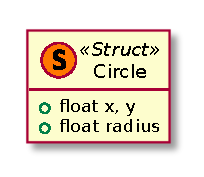
\includegraphics[width=6cm]{archivos/circleuml}
	\caption{Estructura básica de un círculo}
	\label{fig:circleuml}
\end{figure}

Como podemos ver en el código [\ref{cod:drawcircle}], para dibujar una circunferencia, lo que hacemos es ir de \(0\) a \(2 * \pi\). Esto es trazar una circunferencia completa en radianes. Definimos, no obstante, un incremento variable, que depende de la cantidad de puntos que queremos dibujar. De este modo, si queremos dibujar una circunferencia de 4 puntos, este incremento será \((2 \times \pi) \div 4 = \frac{\pi}{2}\), o lo que es lo mismo, dibujaremos de cuarto en cuarto de circunferencia, dibujando así 4 puntos para completar una circunferencia completa.\\

La operación para determinar la posición del punto es muy básica, e implica simplemente un poco de trigonometría. La posición de cada punto de la circunferencia viene determinada por el ángulo (por el coseno del mismo para la coordenada horizontal y por el seno para la coordenada vertical) multiplicado por el radio y sumada la posición del centro de la circunferencia.\\

Una vez obtenida la posición para un punto de la circunferencia, lo dibujamos usando nuestra función del motor para dibujar puntos, que se encarga además de comprobar que el punto esté dentro de los límites de pantalla, y nos permite además pasarle parámetros para el color y el tamaño del punto (blanco y de un píxel para el ejemplo).\\

\begin{lstlisting}[style=C-color, caption={Algoritmo básico de dibujado de circunferencias},label=cod:drawcircle]
void DotTunnelDemo::DrawCircle(const Circle &c)
{
    const float increment = (2 * Fast::PI) / float(pointsPerCircle);
    int x, y;

    for (float angle = 0, n = 2 * Fast::PI; angle < n; angle += increment)
    {
        x = cos(angle) * c.radius + c.x;
        y = sin(angle) * c.radius + c.y;
        
        RenderDot(x, y, Pixel(255), 1);
    }
}
\end{lstlisting}

Una vez podemos dibujar círculos, llega el momento de poder gestionar una serie de círculos y su ciclo de vida (creación, actualizaciones periódicas con radio creciente y destrucción alcanzado un cierto tamaño).\\

Para ello primero debemos preguntarnos, ¿cómo se comporta nuestro túnel? La respuesta es que para la estructura del túnel, lo que queremos es ir añadiendo nuevos círculos al principio del túnel y vamos eliminando los círculos que están al final del túnel cuando alcanzan cierto tamaño. Así pues, esta es una estructura FIFO (\emph{first-in, first-out}) o el primer elemento en crearse es el primer elemento en borrarse. Podríamos pensar que con usar una estructura de cola (\lstinline{std::queue}\footnote{\url{https://en.cppreference.com/w/cpp/container/queue}}) nos bastaría, sin embargo, una cola sólo permite crear un nuevo elemento al final de la estructura y borrarlo al principio, y además no permite el acceso a los elementos intermedios (que nosotros necesitamos para poder actualizarlos).\\

Por suerte, no obstante, hay una estructura similar que cumple todos los requisitos que necesitamos: \lstinline{std::deque}\footnote{\url{https://en.cppreference.com/w/cpp/container/deque}} (\emph{double-ended queue}). Aunque el nombre puede resultar algo extraño (cola con doble final), ¡esta estructura satisface coste constante para todas las operaciones que necesitamos! El coste de la inserción y borrado de elementos son constantes al principio y al final de la cola, y además el acceso aleatorio (acceso a un elemento cualquiera de la cola) es también constante. Por tanto, usaremos esta estructura para contener los círculos que formarán nuestro túnel.\\

\begin{lstlisting}[style=C-color, caption={Inserción y eliminación de círculos},label=cod:populatecirclequeue]
void DotTunnelDemo::PopulateCircleQueue()
{
    if (circles.front().radius > minCircleRadius)
    {
        circles.push_front(defaultCircle);
    }
    if (circles.back().radius > maxCircleRadius)
    {
        circles.pop_back();
    }
}
\end{lstlisting}

Como podemos ver en el código [\ref{cod:populatecirclequeue}], usando esta estructura es muy sencillo añadir y eliminar elementos de nuestro túnel. La lógica que seguimos es: si el último círculo que ha sido añadido alcanza cierto tamaño, entonces añadimos un nuevo círculo al túnel. Del mismo modo, cuando el círculo que más tiempo lleva en la cola alcanza cierto tamaño, es eliminado. Cabe notar que para añadir nuevas circunferencias a la cola, se hace una copia de una instancia que creamos en la inicialización del programa, y que contiene los valores de creación de un círculo por defecto. Además, para que este código funcione correctamente, debe haber al menos un elemento previamente insertado en la cola, es decir, no puede estar vacía. Es por eso que durante la inicialización de la demo también se añade un círculo a la cola, copiado de la instancia por defecto.\\

\begin{lstlisting}[style=C-color, caption={Actualización del túnel},label=cod:updatecirclequeue,escapechar=|]
void DotTunnelDemo::UpdateCircleQueue(float deltaTime)
{
    for (auto c : circles)
    {
        EraseCircle(c);|\label{line:erasecircle}|
    }

    PopulateCircleQueue();

    for (auto &c : circles)
    {
        UpdateCircle(c, deltaTime);|\label{line:updatecircle}|
        DrawCircle(c);
    }
}
\end{lstlisting}

Una vez que podemos dibujar círculos [\ref{cod:drawcircle}] y tenemos una estructura que representa nuestro túnel sobre la que podemos insertar y eliminar elementos [\ref{cod:populatecirclequeue}], llega el momento de dibujar nuestro túnel en pantalla, el proceso es bastante sencillo [\ref{cod:updatecirclequeue}].\\

Lo primero que hacemos es recorrer todos los círculos que conforman el túnel y borrarlos en pantalla, en la línea [\ref{line:erasecircle}]. Es importante notar que esta función no está eliminando los círculos de la cola, si no que simplemente \emph{borra en pantalla}. Internamente esta función llama a la función de dibujado [\ref{cod:drawcircle}] pero con una copia del círculo en color negro. Así, lo que hacemos al inicio de cada actualización es borrar los círculos \emph{que se dibujaron en el fotograma anterior}, previo a la actualización de los valores de los círculos. De este modo, en lugar de tener que poner a negro todos píxeles de la pantalla (que en alta definición son más de un millón), ponemos a negro sólo aquellos píxeles que fueron modificados en el fotograma anterior (que son cientos de píxeles, pero no miles o millones). Al borrar de este modo, se produce una gran optimización.\\

Tras haber borrado la pantalla, llamamos a la función [\ref{cod:populatecirclequeue}], que puede añadir o eliminar círculos del túnel si se cumplen las condiciones necesarias.\\

A continuación, actualizamos (línea [\ref{line:updatecircle}]) y redibujamos todos los círculos en pantalla. Actualmente, la actualización de un píxel es un proceso muy sencillo que consiste simplemente en ir aumentando el radio de cada círculo a lo largo del tiempo, en función de su radio anterior y una velocidad ajustable por el usuario (\lstinline{c.radius += c.radius * deltaTime * radiusVelocity;}).\{\\

El resultado de todo lo aplicado hasta ahora se puede ver en la figura [\ref{fig:basicdottunnel}].\\

\begin{figure}[h]
	\centering
	\includegraphics[width=10cm]{archivos/basicdottunnel}
	\caption{Túnel de puntos básico}
	\label{fig:basicdottunnel}
\end{figure}

Ahora todo lo que nos queda por hacer es dotar de movimiento al túnel, es decir, que no sólo los círculos aumenten de radio, si no que su posición también varíe. No obstante, no es necesario modificar la posición de los círculos una vez han sido creados, basta con que el centro de cada círculo esté desplazado en cuanto a posición con respecto al círculo anterior en su momento de creación. En otras palabras, cada círculo se crea en una posición distinta con respecto al punto de creación del círculo anterior, pero el centro del círculo no se modifica posterior a su creación. Aunque pueda resultar curioso, no es necesario mover el centro del círculo una vez creado, basta con ir haciendo el radio progresivamente más grande para crear una sensación de movimiento convincente.\\

Así pues, tan solo necesitamos crear cada círculo con una posición distinta pero coherente con respecto a la anterior, para dar sensación de continuidad. ¿Cómo podemos hacer esto?\\

No podemos decidir las direcciones de forma aleatoria, pues de este modo el movimiento no parecerá coherente. Cabe la posibilidad, no obstante, de seguir direcciones que se deciden aleatoriamente cada cierto tiempo, pero que se mantienen fijas durante un intervalo. Si hacemos esto el movimiento tendría coherencia pero aún así parecería poco natural cada vez que cambiáramos de dirección, pudiéndose producir cambios de dirección bruscos. Una posibilidad ante esto es interpolar la dirección actual con la dirección futura, de modo que los cambios de dirección queden suavizados. Pero aun así surge un problema más, no podemos controlar si el túnel se sale de los límites de la pantalla. Podríamos hacer entonces que si el túnel está cerca del límite de la pantalla, la nueva dirección elegida fuera hacia el centro de la pantalla. Aunque esto podría causar sensación de que cuando el túnel se acerca al límite de la pantalla rebota... Podríamos seguir con este modelo, a partir de direcciones o movimientos aleatorios, pues es factible, pero el código y la cantidad de situaciones con las que hay que lidiar para que el resultado parezca natural aumenta en  complejidad por momentos.\\

Fue por ello que cuando estaba pensando en cómo implementar este efecto, descarté esta opción. Pensando en otras opciones se me ocurrió la que sería la definitiva, construir un camino a partir de un punto que gira en torno a una "órbita" virtual que a su vez "orbita" en torno a otros puntos. Un poco de forma parecida a como orbitan los planetas, que si bien lo hacen bajo rutas perfectamente definidas, las combinaciones de órbitas a distintas velocidades dan resultado a trayectorias coherentes pero difíciles de predecir desde el punto de vista terráqueo [\ref{fig:cassini}].\\

\begin{figure}[h]
	\centering
	\includegraphics[width=8cm]{archivos/cassini}
	\caption{Órbitas de los planetas vistas desde la Tierra (por Giovanni Cassini) - Fuente: \href{https://es.wikipedia.org/wiki/Teoría_heliocéntrica\#/media/File:Cassini_apparent.jpg}{Wikipedia}}
	\label{fig:cassini}
\end{figure}

Así, con el modelo geocéntrico en mente, me dispuse a crear una clase que fuera capaz de emular este tipo de movimiento: controlado pero difícil de predecir.\\

me queda decir como hice el camino de turbulencia, luego toca explicar el refinamiento (color, opacidad, rotacion e input) y ya por ultimo queda mostrar los resultados, tras ello me pondré con los tests de rendimiento

\subsection{Refinamiento}

rgerg
sgsdgsfdh

sg

drga

rg

ergregearg

rgerg

\subsection{Resultado}

rgerg
sgsdgsfdh

sg

drga

rg

ergregearg

rgerg

\section{RotoZoom}

\subsection{Investigación inicial}

rgerg
sgsdgsfdh

sg

drga

rg

ergregearg

rgerg

\subsection{Planteamiento formal}

rgerg
sgsdgsfdh

sg

drga

rg

ergregearg

rgerg

\subsection{Implementación}

rgerg
sgsdgsfdh

sg

drga

rg

ergregearg

rgerg

\subsection{Refinamiento}

rgerg
sgsdgsfdh

sg

drga

rg

ergregearg

rgerg

\subsection{Resultado}

rgerg
sgsdgsfdh

sg

drga

rg

ergregearg

rgerg

\section{Deformaciones de imagen}

\subsection{Investigación inicial}

rgerg
sgsdgsfdh

sg

drga

rg

ergregearg

rgerg

\subsection{Planteamiento formal}

rgerg
sgsdgsfdh

sg

drga

rg

ergregearg

rgerg

\subsection{Implementación}

rgerg
sgsdgsfdh

sg

drga

rg

ergregearg

rgerg

\subsection{Refinamiento}

rgerg
sgsdgsfdh

sg

drga

rg

ergregearg

rgerg

\subsection{Resultado}

rgerg
sgsdgsfdh

sg

drga

rg

ergregearg

rgerg

\section{Plasma}

\subsection{Investigación inicial}

rgerg
sgsdgsfdh

sg

drga

rg

ergregearg

rgerg

\subsection{Planteamiento formal}

rgerg
sgsdgsfdh

sg

drga

rg

ergregearg

rgerg

\subsection{Implementación}

rgerg
sgsdgsfdh

sg

drga

rg

ergregearg

rgerg

\subsection{Refinamiento}

rgerg
sgsdgsfdh

sg

drga

rg

ergregearg

rgerg

\subsection{Resultado}

rgerg
sgsdgsfdh

sg

drga

rg

ergregearg

rgerg


\section{Planos infinitos}

\subsection{Investigación inicial}

rgerg
sgsdgsfdh

sg

drga

rg

ergregearg

rgerg

\subsection{Planteamiento formal}

rgerg
sgsdgsfdh

sg

drga

rg

ergregearg

rgerg

\subsection{Implementación}

rgerg
sgsdgsfdh

sg

drga

rg

ergregearg

rgerg

\subsection{Refinamiento}

rgerg
sgsdgsfdh

sg

drga

rg

ergregearg

rgerg

\subsection{Resultado}

rgerg
sgsdgsfdh

sg

drga

rg

ergregearg

rgerg


\section{Geometría}


\subsection{Investigación inicial}

rgerg
sgsdgsfdh

sg

drga

rg

ergregearg

rgerg

\subsection{Planteamiento formal}

rgerg
sgsdgsfdh

sg

drga

rg

ergregearg

rgerg

\subsection{Implementación}

rgerg
sgsdgsfdh

sg

drga

rg

ergregearg

rgerg

\subsection{Refinamiento}

rgerg
sgsdgsfdh

sg

drga

rg

ergregearg

rgerg

\subsection{Resultado}

rgerg
sgsdgsfdh

sg

drga

rg

ergregearg

rgerg
